\documentclass[../article.tex]{subfiles} % 继承主文档配置

\graphicspath{{../../images}} % 设置图片路径

\begin{document}

\section{研究的主要内容}
\subsection{单元格物理坐标定位}

在表格结构识别中,单元格物理坐标用于精确描述单元格在图像中的位置,合适的单元格物理坐标的表示方法为表格结构识别提供了精确的定位基础,尤其是在表格结构重建和数据提取过程中,它们能够确保单元格位置的准确性,也为后续的单元格逻辑坐标定位提供了基础。

\subsection{基于单元格的细粒度分割模型的构建}

传统的表格结构提取方法主要依赖于线段检测和几何模型推理,这些方法虽然在处理标准化表格时表现良好,但在面对形变严重的表格时,其局限性逐渐显现。尤其是直线检测算法,通常通过霍夫变换等技术检测图像中的直线,以识别表格的行和列。尽管这种方法在结构清晰的表格中运作良好,但一旦表格因拍照或扫描产生了形变,行列的线条可能出现弯曲或断裂,从而导致算法无法有效识别,最终影响表格结构的提取精度。于是,有的研究转向通过四个关键角点来表示单元格物理坐标。

\begin{figure}[H]
    \centering
    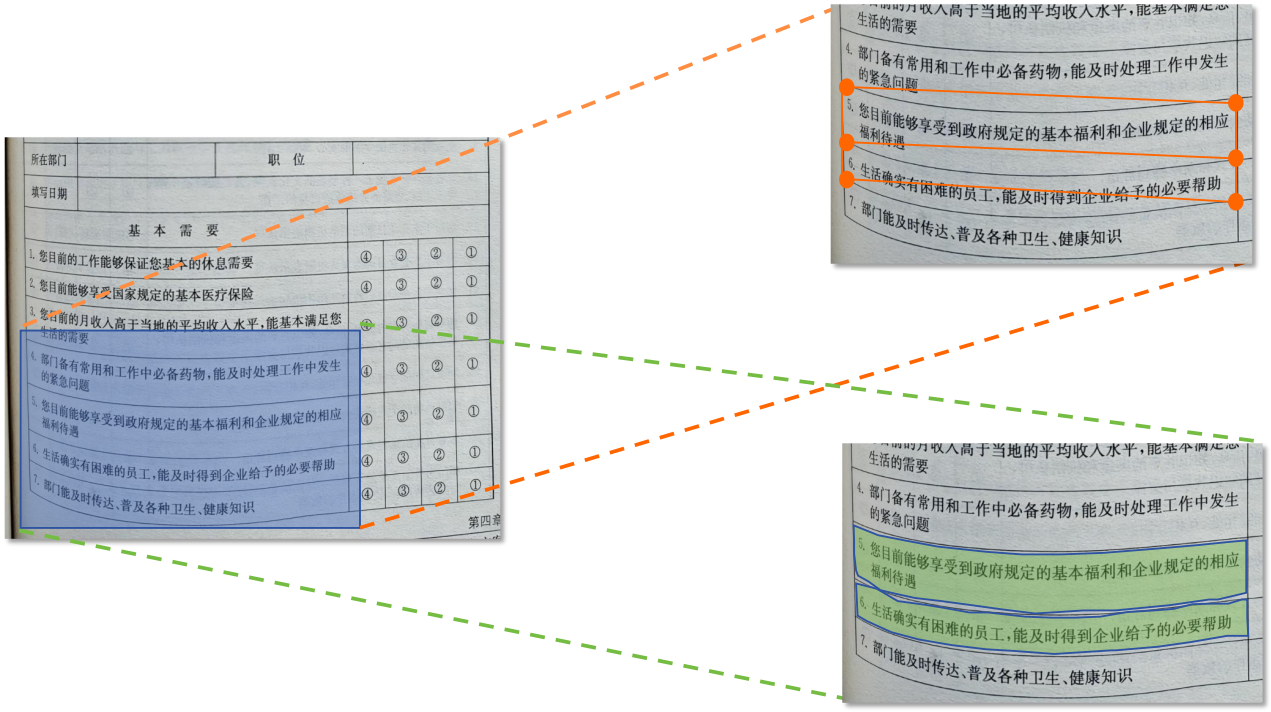
\includegraphics[width=0.9\textwidth]{point.png}
    \caption{关键点检测与图像分割}
    \label{fig:p}
\end{figure}

然而,基于关键点推理的模型也存在一定局限性,如图\ref{fig:p},单元格的边界可能形变过于严重,导致定位出得到的单元格在后期的OCR识别丢失了大量信息,也给逻辑坐标还原带来了巨大的挑战。这种情况下,单纯依靠几何形状的描述已无法满足实际需求,为了解决这些问题,本课题关注基于图像分割的技术。与关键点推理模型的方式不同,图像分割通过对图像进行像素级的处理,能够捕捉到每个单元格的边界信息,并保留更多细节。特别是在处理复杂形状和形变严重的情况下,图像分割算法展现出强大的能力,这种细粒度的识别方法能最大程度上保留单元格的内容信息区域。

\subsection{单元格逻辑坐标定位}

与单元格物理坐标不同,单元格逻辑坐标主要描述单元格之间的相对位置和从属关系,通常用于表示表格的布局结构和单元格之间的逻辑关系。通过获取单元格逻辑坐标,可以更加清楚的了解表格中单元格之间的关系,如单元格本身的行列信息、单元格的合并信息、单元格的跨行跨列信息等。这对于表格结构映射还原具有重要意义。

\subsection{表格结构映射还原}

表格重组是表格识别中的一个辅助步骤,目的是通过物理坐标和逻辑坐标的结合,将表格中的单元格从图像中的位置恢复为规整的、标准化的表格布局。这一过程帮助系统将单元格准确排列,确保不同单元格之间的空间和结构关系正确。


\end{document}